Now that the requirements necessary to build the system have been formulated, potential solutions to fulfil the list of requirements from Chapter \ref{ch:chapter3} for each aspect of the system can now be analysed before a final solution can be chosen. The first section of this chapter will focus on different solutions for the system's pipeline, starting with the offline feature extraction phase, followed by the online retrieval phase, and ending with the database pre-processing phase. The second section will focus on general design decisions such as the programming language, the type of interface and the type of videos to use. These two sections will be used to outline the final chosen solutions for each aspect of the system before concluding with a development plan.

\section{Pipeline Design Analysis}

In order to chose a global design solution for the system, it is easier to break down the system's pipeline into different phases and review the numerous potential designs for each of these phases. The system pipeline can be split into three different phases, as shown in Figure \ref{fig:basic-cbvr-diagram}:

\begin{itemize}
    \item \textbf{Offline Feature Extraction Phase}. This phase corresponds to the ``training'' phase of the system, where features are extracted from each video in the database and then stored in data files for the retrieval phase.
    \item \textbf{Online Retrieval Phase}. This phase is affiliated to the ``training'' phase of the system, where a single video query is matched to one of the database videos by extracting the same features from the previous phase and comparing them to the stored features.
    \item \textbf{Database Pre-processing Phase}. This is an optional phase where the database videos are processed before the offline feature extraction phase to improve the accuracy and speed of the database videos feature extraction.
\end{itemize}

\begin{figure}[h]
\centerline{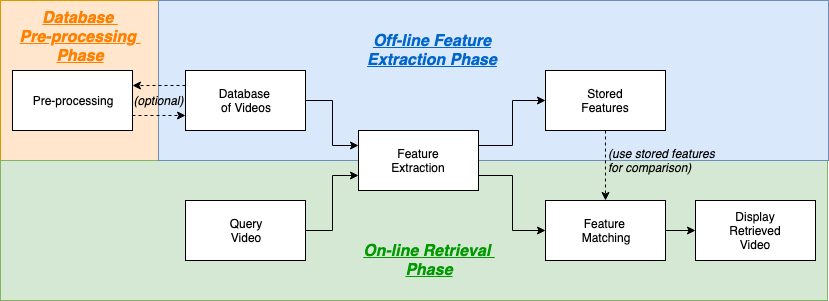
\includegraphics[width=\textwidth]{figures/design/basic_cbvr_phases.png}}
\caption{\label{fig:basic-cbvr-diagram}Basic CBVR system diagram.}
\end{figure}

\begin{comment}
Explore possible options for different sections of the system, such as:
    \begin{itemize}
        \item types of features to extract (why static colour features and not object/motion features) - histograms are very popular with videos, calculations are easier, implementation is easier, results are as efficient
        \item types of learning models (histogram matching, BoW-approach VS Neural Network)
    \end{itemize}
\end{comment}

\subsection{Offline Feature Extraction Phase}

todo

\subsection{Online Retrieval Phase}

todo

\subsection{Database Pre-Processing Phase}

todo

\section{General Project Design}

Now that the design choices regarding the system pipeline have been made, general system choices such as the programming language, the interface, the feature storage and the database videos can be inspected.

\subsection{Programming Language}

The programming language is one of the most important aspects when it comes to designing and later implementing the system as it is the medium used to transform the system from design to implementation. However, choosing between 250 different programming languages \cite{tiobe} can be a tricky exercise, which is why multiple views have to be reviewed before a programming language can be chosen. Multiple criteria are considered to justify the choice of the programming languages, including the availability of computer vision-related functions, the runtime speed, the readability and the personal preference.\\

The first element to consider when choosing a programming language for this type of project is the availability of functions for video manipulation and computer vision-related operations. Indeed, using high-level functions to, e.g. read videos or generate histograms is primordial to avoid spending time manually implementing each of these functionalities and to instead devote more time on implementing high-level concepts to complete the pipeline. Some languages such as MATLAB and Python (with mainstream third-party libraries) allow for native manipulation of images/videos and offer collections of computer vision functions. For other programming languages, libraries can be used. The most popular library is OpenCV\footnote{OpenCV, \url{https://opencv.org/}}, which offers functions for real-time computer vision applications. This library supports all the main operating systems (Linux, macOS, Windows, etc.) and although it was mainly designed for C/C++, it contains bindings for the main general-purpose programming languages such as Python, Java, C\#, Javascript, Haskell and MATLAB.\\

Among the previously mentioned programming languages, C/C++ are the fastest languages,
according to ``Benchmark Games''\footnote{Benchmark Games: \url{https://benchmarksgame-team.pages.debian.net/benchmarksgame/}}, followed by Java, Javascript and Python, which is considerably slower than the aforementioned programming languages. However, Python can be extended with languages such as C/C++ with ease. This means that coupling Python with the OpenCV library that is initially written in C++ allows the Python code to execute as fast as the original C++ code since it is the actual OpenCV C++ code that is running in the background. Furthermore, Python has an extensive set of third-party libraries that add powerful functionalities to the language, such as Numpy, SciPy and MatplotLib that add mathematical and scientific functions that can compete with MATLAB's native functions. Finally, of all the specified programming languages, Python is the favoured one in terms of personal preference, familiarity, and experience. Therefore, the relatively slower execution speeds of Python that are cancelled out when using OpenCV, coupled with the personal preference for Python, make Python the obvious programming language choice for this project.\\

TODO: add table of pros and cons in appendix

\subsection{Interface}

Now that is has been decided that Python will be the programming language used to implement the system, the next decision is the type of interface that will be used to present the results. Although it was specified

interface choice (why CLI VS GUI?): time constraints and no users, goal of this project is to research efficient results, not create a commercial product

\subsection{Feature Storing}

txt files VS dat files VS binary files

\subsection{Database videos}

types of videos in databases (why short videos VS movies, cartoons/stop-motion pictures)

\section{Chosen Solution}

include a high-level diagram of system excluding detail (all DB videos in system, single query video in system, matching video output)

\section{Development Plan}

plan with time constraints in mind

\section{Summary}

summarise section
